\documentclass{article}
\usepackage{amsmath}
\usepackage{graphicx}
\usepackage[utf8]{inputenc}

\title{3D Coordinate System}
\author{yuehan9.wu@gmail.com}
\date{\today}

\begin{document}
\maketitle
\section*{Object Space}
Also known as local space. Postion is encoded in model data such as gltf.
\[(AB)^{T} = (B)^{T}(A)^{T}\]
\[(A^{-1})^{T} = (A^{T})^{-1}\]
\[T(t_{x}, t_{y}, t_{z}) = \begin{bmatrix}
    1 &0 &0 &t_{x} \\
    0 &1 &0 &t_{y} \\
    0 &0 &1 &t_{z} \\
    0 &0 &0 &1
\end{bmatrix}\]
\[R_{x}(\phi) = \begin{bmatrix}
    1 &0 &0 &0 \\
    0 &\cos(\phi) &-\sin(\phi) &0 \\
    0 &\sin(\phi) &\cos(\phi) &0 \\
    0 &0 &0 &1
\end{bmatrix}\]
\[R_{y}(\phi) = \begin{bmatrix}
    \cos(\phi) &0 &\sin(\phi) &0 \\
    0 &1 &0 &0 \\
    -\sin(\phi) &0 &\cos(\phi) &0 \\
    0 &0 &0 &1
\end{bmatrix}\]
\[R_{z}(\phi) = \begin{bmatrix}
    \cos(\phi) &-\sin(\phi) &0 &0 \\
    \sin(\phi) &\cos(\phi) &0 &0 \\
    0 &0 &1 &0 \\
    0 &0 &0 &1
\end{bmatrix}\]
\[S(\lambda ) = \begin{bmatrix}
    \lambda_{x} &0 &0 &0 \\
    0 &\lambda_{y} &0 &0 \\
    0 &0 &\lambda_{z} &0 \\
    0 &0 &0 &1
\end{bmatrix}\]
\[X = T(t)R = \begin{bmatrix}
    a_{00} &a_{01} &a_{02} &t_{x} \\
    a_{10} &a_{11} &a_{12} &t_{y} \\
    a_{20} &a_{21} &a_{22} &t_{z} \\
    0 &0 &0 &1
\end{bmatrix}\]

\section*{Camera Space}
It transforms right vector (world space) into \((1, 0, 0)\) as,
\[V\begin{bmatrix}
    r_{x} \\ r_{y} \\ r_{z} \\ 0
\end{bmatrix}=\begin{bmatrix}
    1 \\ 0 \\ 0 \\ 0
\end{bmatrix}\]
It transforms up vector (world space) into \((0, 1, 0)\) as,
\[V\begin{bmatrix}
    u_{x} \\ u_{y} \\ u_{z} \\ 0
\end{bmatrix}=\begin{bmatrix}
    0 \\ 1 \\ 0 \\ 0
\end{bmatrix}\]
It transforms negative view vector (world space) into \((0, 0, 0)\) as,
\[V\begin{bmatrix}
    v_{x} \\ v_{y} \\ v_{z} \\ 0
\end{bmatrix}=\begin{bmatrix}
    0 \\ 0 \\ 1 \\ 0
\end{bmatrix}\]
It transforms eye location (world space) into \((0, 0, 0, 1)\) as,
\[V\begin{bmatrix}
    e_{x} \\ e_{y} \\ e_{z} \\ 1
\end{bmatrix}=\begin{bmatrix}
    0 \\ 0 \\ 0 \\ 1
\end{bmatrix}\]
To put together,
\[V\begin{bmatrix}
    r_{x} &u_{x} &v_{x} &e_{x} \\
    r_{y} &u_{y} &v_{y} &e_{y} \\
    r_{z} &u_{z} &v_{z} &e_{z} \\
    0 &0 &0 &1
\end{bmatrix}=\begin{bmatrix}
    1 &0 &0 &0 \\
    0 &1 &0 &0 \\
    0 &0 &1 &0 \\
    0 &0 &0 &1
\end{bmatrix}\]
\[V\begin{bmatrix}
    1 &0 &0 &e_{x} \\
    0 &1 &0 &e_{y} \\
    0 &0 &1 &e_{z} \\
    0 &0 &0 &1
\end{bmatrix}\begin{bmatrix}
    r_{x} &u_{x} &v_{x} &0 \\
    r_{y} &u_{y} &v_{y} &0 \\
    r_{z} &u_{z} &v_{z} &0 \\
    0 &0 &0 &1
\end{bmatrix}=\begin{bmatrix}
    1 &0 &0 &0 \\
    0 &1 &0 &0 \\
    0 &0 &1 &0 \\
    0 &0 &0 &1
\end{bmatrix}\]
\[V=\begin{bmatrix}
    r_{x} &u_{x} &v_{x} &0 \\
    r_{y} &u_{y} &v_{y} &0 \\
    r_{z} &u_{z} &v_{z} &0 \\
    0 &0 &0 &1
\end{bmatrix}^{-1}\begin{bmatrix}
    1 &0 &0 &e_{x} \\
    0 &1 &0 &e_{y} \\
    0 &0 &1 &e_{z} \\
    0 &0 &0 &1
\end{bmatrix}^{-1}\]
\[V=\begin{bmatrix}
    r_{x} &r_{y} &r_{z} &0 \\
    u_{x} &u_{y} &u_{z} &0 \\
    v_{x} &v_{y} &v_{z} &0 \\
    0 &0 &0 &1
\end{bmatrix}\begin{bmatrix}
    1 &0 &0 &-e_{x} \\
    0 &1 &0 &-e_{y} \\
    0 &0 &1 &-e_{z} \\
    0 &0 &0 &1
\end{bmatrix}\]

\section*{Projection Space}
\subsection*{Orthographics}
Parallel lines keep parallel.
\[P_{o } = \begin{bmatrix}
    1 &0 &0 &0 \\
    0 &1 &0 &0 \\
    0 &0 &0 &0 \\
    0 &0 &0 &1
\end{bmatrix}\]
In OpenGL, the general form should take an AABB into consideration.
The volume is guarded by six-tuple, \((left, right, bottom, top, near, far)\)
\[P_{o } = S(s)T(t)= \begin{bmatrix}
    \frac{2}{r-l} &0 &0 &0 \\
    0 &\frac{2}{t-b} &0 &0 \\
    0 &0 &\frac{2}{f-n} &0 \\
    0 &0 &0 &1
\end{bmatrix}\begin{bmatrix}
    1 &0 &0 &-\frac{l+r}{2} \\
    0 &1 &0 &-\frac{b+t}{2} \\
    0 &0 &1 &-\frac{n+f}{2} \\
    0 &0 &0 &1
\end{bmatrix}\]
\subsection*{Perspective}
Near object looks larger.
Assume we put camera at origin and the project plane \((0, 0, -n)\)
\[v{'} = Pv = \begin{bmatrix}
    1 &0 &0 &0 \\
    0 &1 &0 &0 \\
    0 &0 &1 &0 \\
    0 &0 &-1/n &0
\end{bmatrix}\begin{bmatrix}
    x \\ y \\ z \\ 1
\end{bmatrix} = \begin{bmatrix}
    x \\ y \\ z \\ -z/n
\end{bmatrix}\]
If we do perspective division,
\[\begin{bmatrix}
    x{'} \\ y{'} \\ z{'} \\ w'
\end{bmatrix} = \begin{bmatrix}
    -nx/z \\ -ny/z \\ -n \\ -z/n
\end{bmatrix}\]
Take a frustum \((l, r, b, t, n, f)\) into consideration,
\begin{equation}
    \begin{cases}
        kr+b = 1 \\
        kl+b = -1
    \end{cases}
    \begin{cases}
        k = \frac{2}{r-l} \\
        b = -\frac{r+l}{r-l}
    \end{cases}
\end{equation}
\begin{equation}
    \begin{cases}
        x_{n} = \frac{2x_{p}}{r-l} - \frac{r+l}{r-l} \\
        y_{n} = \frac{2y_{p}}{t-b} - \frac{t+b}{t-b} \\
    \end{cases}
\end{equation}
\[x_{n}=\frac{2x_{p}}{r-l} - \frac{r+l}{r-l}
= \frac{2n\frac{x_{e}}{-z_{e}}}{r-l} - \frac{r+l}{r-l}
= \frac{2nx_{e}}{(r-l)(-z_{e})} - \frac{r+l}{r-l}\]
\[=\frac{\frac{2n}{r-l}x_{e}}{-z_{e}}+\frac{\frac{r+l}{r-l}z_{e}}{-z_{e}}
=(\frac{2n}{r-l}x_{e}+\frac{r+l}{r-l}z_{e})/-z_{e}\]
\[z_{n}=z_{c}/w_{c}=\frac{Az_{e}+Bw_{e}}{-z_{e}}\]
In eye space, \(w_{e}\) equals 1. Therefore,
\[z_{n}=z_{c}/w_{c}=\frac{Az_{e}+B}{-z_{e}}\]
\begin{equation}
    \begin{cases}
        \frac{An+B}{-n} = -1 \\
        \frac{Af+B}{-f} = 1
    \end{cases}
    \begin{cases}
        A = -\frac{f+n}{f-n} \\
        B = -\frac{2fn}{f-n}
    \end{cases}
\end{equation}
In summary,
\[\begin{bmatrix}
    x_{c} \\ y_{c} \\ z_{c} \\ w_{c}
\end{bmatrix}=\begin{bmatrix}
   \frac{2n}{r-l} &0 &\frac{r+l}{r-l} &0 \\
   0 &\frac{2n}{t-b} &\frac{t+b}{t-b} &0 \\
   0 &0 &-\frac{f+n}{f-n} &-\frac{2fn}{f-n} \\
   0 &0 &-1 &0
\end{bmatrix}\begin{bmatrix}
    x_{e} \\ y_{e} \\ z_{e} \\ w_{e}
\end{bmatrix}=\begin{bmatrix}
    \frac{2n}{r-l}x_{e}+\frac{r+l}{r-l}z_{e} \\
    \frac{2n}{t-b}y_{e}+\frac{t+b}{t-b}z_{e} \\
    -\frac{f+n}{f-n}z_{e}-\frac{2fn}{f-n} \\
    -z_{e}
\end{bmatrix}\]
\begin{center}
    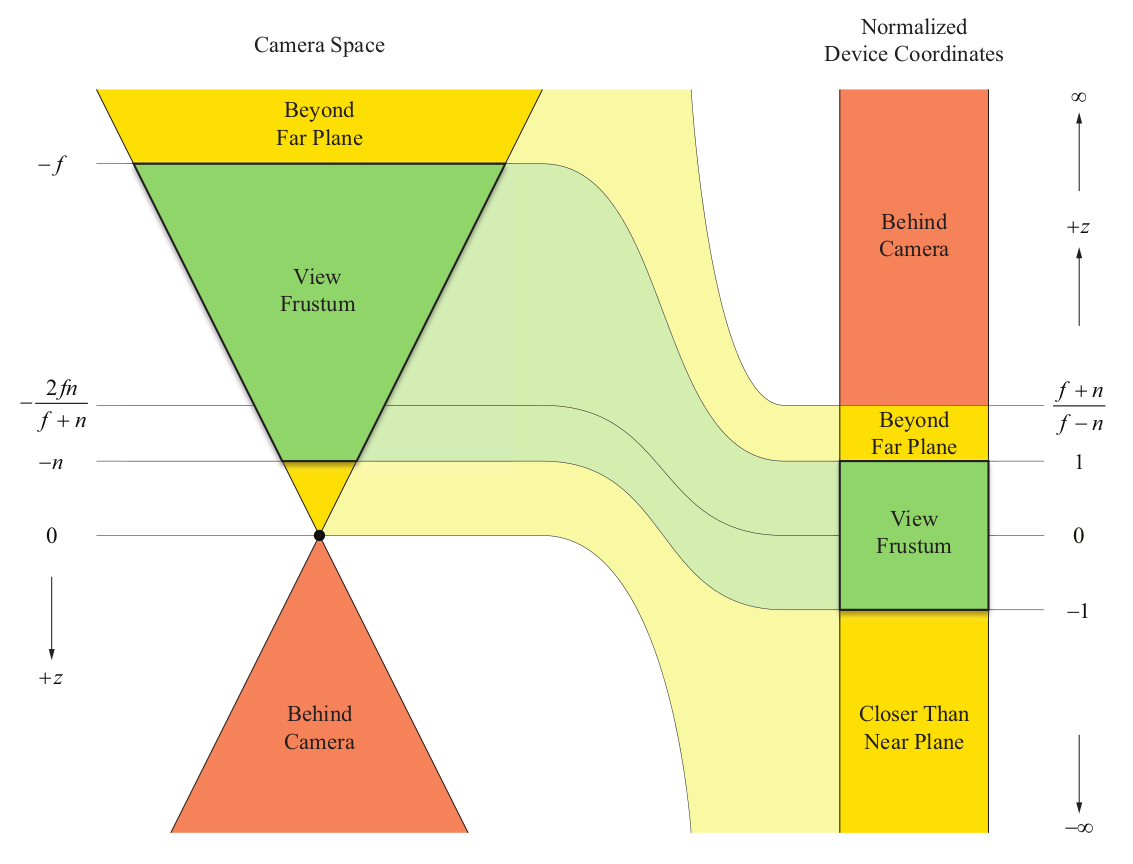
\includegraphics[scale=0.25]{./ndc.png}
\end{center}

\section*{Clip Space}
The output from vertex shader by \((x_{c}, y_{c}, z_{c}, w_{c})\). The clip volume
is given as follow:
\[-w_{c} <= x_{c} <= w_{c}\]
\[-w_{c} <= y_{c} <= w_{c}\]
\[-w_{c} <= z_{c} <= w_{c}\]
If a primitive is completely outside the clipping volume, it is discarded.
If a primitive is partly inside the clipping volume, new vertices are generated.

\section*{NDC Space}
Undergo perspective division as follow:
\[(\frac{x_{c}}{w_{c}}, \frac{y_{c}}{w_{c}}, \frac{z_{c}}{w_{c}}, w_{c})\]
It is called normalized device coordinate, as it will be in below range:
\[-1 <= x_{n} <= 1\]
\[-1 <= y_{n} <= 1\]
\[-1 <= z_{n} <= 1\]

\end{document}